\lfoot{Autor: Fitim Faiku}
\subsection{Fahrkomfortanalyse}


Da die Bewertung der einzelnen Fahrer durch den Fahrgast erfolgt ist jedem klar.
Diese Bewertung fällt meistens aus den Faktoren wie stark ein Fahrer beschleunigt und in welcher Geschwindigkeit er um eine Kurve fährt.
Um einen KFZ-Einsteiger mit möglichst Informativen Daten zu \"bewerten\" haben wir uns einen Kammschen Kreis als Hilfe genommen.

\subsubsection{Kammscher Kreis }
Ein Kammsher Kreis ist ein ein Kreis in dem durch Polarkoordinaten die Extremwerte einer Fahrt eingezeichnet sind.
Der Kreis ist so aufgebaut, dass in Norden de Bremskräfte angezeigt werden, in Süden alle Beschleunigungen, im Westen die Rechtskurven und Osten die Linkskurven.
Es ist also alles verkehrt.
\begin{figure}[!htb]\centering
	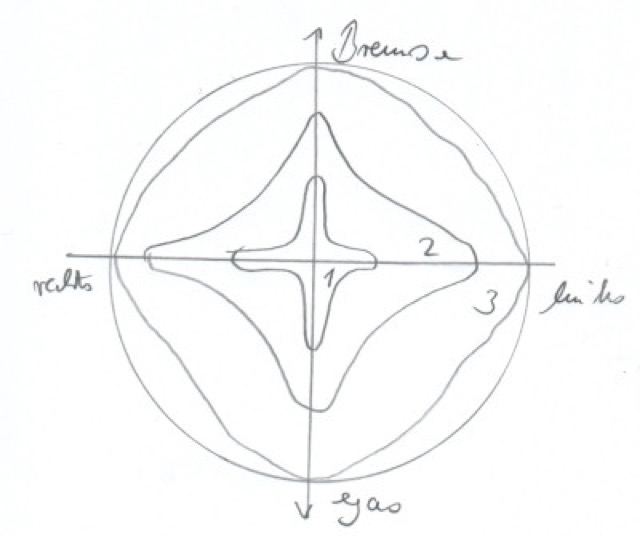
\includegraphics[width=0.5\textwidth]{images/kammsherkreis}
	\caption{Kammsherkreis \cite{FAIF.CH3-fahrkomfortanalyse.KammscherKreis}}\label{Fig:Kammsher-Kreis}
\end{figure}

\subsubsection{Implementierung}
Um diesen Kammschen Kreis richtig darzustellen haben wir uns die Klasse canvas als Hilfe genommen, wobei die von Graphics erbt und wir somit auf einer Fläche zeichnen können.
Mittels Canvas konnten wir zufällig generierte 0-360grad Winkel und Radien erstellen und diese dann in Polarkoordinaten umrechnen.
Somit konnten wir alle generierten werte Darstellen. 

\lstinputlisting[caption=Runden-Methode, style=javastyle]{code/Runden.java}

Bei der Methode Runden nehmen wir alle Winkel auf und runde sie auf oder ab in 5er Schritten.
\newline 


\lstinputlisting[caption=Draw, style=javastyle]{code/ChartView.java}
Um den Kammshen-Kreis zu zeichnen habe ich die OnDraw Methode ueberschrieben, weiters speichere ich alle generierten Werte in einer Liste welche in einer For-Schleife gezeichnet werden.